\matlab is a popular numeric programming language, used by millions of
scientists, engineers as well as students worldwide\cite{MatlabGrowth}.  \matlab
programmers appreciate the high-level matrix operators,  the fact that
variables and types do not need to be declared, the large number of library and
builtin functions available, and the interactive style of program development
available through the IDE and the interpreter-style read-eval-print loop.
However, even though \matlab programmers appreciate all of the features that
enable rapid prototyping,  their applications are often quite compute intensive
and time consuming. These applications could perform much more efficiently if
they could be easily ported to a high performance computing system.  

On one hand, all the aforementioned characteristics of \matlab make it a very 
user-friendly and thus popular application to develop software among a
non-programmer community. On the other hand, these same characteristics make
\matlab a difficult language to compile statically. Even the de facto standard, 
Mathworks' 
implementation of \matlab is essentially an interpreter with a 
\emph{JIT accelarator}\cite{matlabjit} which is generally slower than statically
compiled languages. GNU Octave, which is a popular open source alternative to  
\matlab and is mostly compatible with \matlab, is also implemented as an
interpreter\cite{Octave}. 
Lack of formal language specification, unconventional semantics
and closed source make it even harder to write a compiler for \matlab.
Furthermore, the use         
of arrays as default data type and the dynamicity of the base types and         
shapes of arrays also make it harder to add support for concurrency in a        
static \matlab compiler.  Mathworks'         
proprietary solution for concurrency is the \emph{Parallel Computing            
Toolbox}\cite{pct}, which allows users to use multicore processors, GPUs        
and clusters. However, this toolbox uses heavyweight worker threads and         
has limited scalability.         

In this thesis, our aim is to provide \matlab's ease of use, to benefit from the 
advantages of static compilation, and to expose scalable concurrency.           
Our solution is \mixten, an open, source-to-source compiler that statically 
compiles \matlab for high performance computing by translating \matlab programs
to \xten\cite{x10}, a language specifically designed for high performance computing
systems. \xten is an                   
object-oriented and statically-typed language which uses cilk-style             
arrays indexed by \emph{Point} objects and rail-backed multidimensional         
arrays, and has been designed with well-defined semantics and high              
performance computing in mind.  The \xten compiler can               
generate C++ or Java code and supports various communication interfaces         
including sockets and MPI for communication between nodes on a parallel         
computing system.                                      

We have concentrated both on providing an efficient translation for the         
sequential core of \xten, as well as providing an effective bridge to           
the concurrency features of \xten. One key way in which we interface          
with concurrency in \matlab is by designing and implementing a                  
translation of the \matlab \texttt{parfor} construct to \xten.  We also                 
introduced concurrency constructs in \matlab analogous to those provided        
in \xten, thus allowing users to further specify fine-grained                   
concurrency in their programs.   

The overall goal of the \mixten project it to allow scientists and              
engineers to write programs in \matlab (or use existing programs already        
written in \matlab), and at the same time enjoy the benefits of high            
performance computing via the \xten system without having to learn a new        
and unfamiliar language.   Also, since the \xten compiler has back-ends         
that can produce both C++ and Java,  \mixten can also be used by systems        
that use \matlab for prototyping and C++ or Java for production.  

%In this thesis we present \mixten, a source-to-source compiler that helps
%to bridge the gap between \matlab, a language familiar to scientists,
%and \xten,  a language designed for high performance computing systems. 
%\mixten statically compiles \matlab programs to \xten and thus
%allows scientists and engineers to write programs in \matlab (or reuse existing 
%programs written in \matlab) and still get the benefits of high 
%performance computing without having to learn a new language or rewriting the
%programs in a different language. Also, systems that
%use \matlab for prototyping and C++ or Java for production, can benefit from
%\mixten by quickly converting \matlab prototypes to C++ or Java programs via 
%\xten. 
%\figref{Fig:flow} shows the flow of compilation from \matlab to
%executable code via \mixten. 
%In particular, this thesis identifies the key 
%challenges in compiling a
%dynamically-typed language like \matlab to a statically-typed object-orinted
%high performance computing language like \xten and our approach to 
%compiling \matlab to \xten.
%\begin{figure}[htbp]                                                            
%\begin{center}                                                                  
%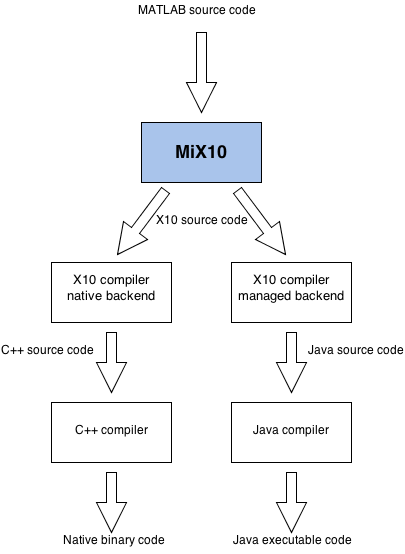
\includegraphics[scale=0.4]{images/mix10_compilation_flow}                             
%\caption {Compilation flow via \mixten}\label{Fig:flow}                    
%\end{center}                                                                    
%\end{figure}     

% Built on top of \mclab frontend and static analysis tools,
% \mixten provides static compilation for \matlab via the C++
%backend for \xten and thus ultimately aims to have better performance even with
%sequential code. 
%uncomment below if tamer+ used
%\mixten also concentrates on readability of the generated \xten
%code to meet the other goal of this thesis, which is to help users port 
%their code from \matlab to \xten.    

\section{Contributions}
  
The major contributions  of this thesis are as follows:

\begin{description}

\item[Identifying key challenges:] We have identified the key challenges
in performing a semantics-preserving efficient translation of \matlab to \xten.

\item[Overall design of \mixten:] We provide the design of a 
source-to-source translator, building upon the \mclab front-end and
analysis toolkits\cite{JesseThesis, TamerPaper}.

\item[Techniques for efficient compilation of \matlab arrays:] Arrays are 
the core of \matlab. All data, including scalar values are represented          
as arrays in \matlab. Efficient compilation of arrays is the key for            
good performance. \xten provides two          
types of array representations for multidimensional arrays: (1)                 
Cilk-styled, region-based arrays and (2) rail-backed arrays. We compare         
and contrast these two array forms for a high performance computing             
language in context of being used as a target language and provide techniques 
to compile \matlab arrays to two different representations of arrays provided 
by \xten.

\item[Analysis to identify variables safe to be declared as \texttt{Long} type:] 
In \matlab all variables are by default of type
\texttt{Double}. In \xten however, certain variable uses, for example, use of a
variable as an array index in an array access operation, require the variable to
be of type \texttt{Long}. We provide an analysis to automatically identify 
variables that can be safely declared to be of type \texttt{Long} without 
affecting the correctness of the generated \xten code. This helps to eliminate
most of, otherwise necessary, typecast operations which our experiments
showed to be a major performance bottleneck in the generated code.      

%\item[\mixten IR design:] In order to provide a convenient
%target for the first level of translation, we have defined a high-level
%\mixten IR.  This IR is used for code generation, \xten specific analyses, 
%code simplifications and transformations.

%\item[Comparison of different kinds of \xten arrays:] version 2.4 of \xten 
%(latest version as of this writing) provides two kinds of multi-dimensional 
%arrays, \emph{region-based} arrays and \emph{rail-backed} arrays.  

\item[Support for concurrency constructs:] \parfor is a \matlab construct that 
allows parallel execution of for loop         
iterations. We provide technique to effectively compile              
\parfor construct to \xten. We also discuss our strategy to handle              
vectorized instructions in a concurrent fashion.  Besides providing support for
existing \matlab concurrency features, we have also introduced \xten like
concurrency constructs in \matlab,                
allowing \matlab programmers to expose fine-grained concurrency in their        
programs.

\item[Code generation strategies for key language constructs:]  There
are some very significant differences between the semantics of \matlab
and \xten.  A key difference is that \matlab is dynamically-typed,
whereas \xten is statically-typed.   Furthermore, the type rules are
quite different, which means that the generated \xten code must include
the appropriate explicit type conversion rules, so as to match the
\matlab semantics.   Other \matlab features, such as multiple returns
from functions, a non-standard semantics for \texttt{for} loops, and a
very general range operator, must also be handled correctly.  We
have also designed and implemented a template-based system that allows us to
generate specialized \xten code for a collection of important \matlab builtin
operations.

\item[isComplex value analysis:] We designed an analysis for identification of 
complex numerical values in a \matlab program. This helped us to extend \mixten
compiler to also generate \xten code for \matlab programs that involve use of
complex numerical values. 

\item[Working implementation and performance results:] We have implemented the 
\mixten compiler over various \matlab compiler tools provided by the \mclab
toolkit.  
In the process we also implemented some enhancements to these existing tools.
We provide performance results for different \xten backends over a set 
of benchmarks and compare them with results from other \matlab compilers
including Mathworks' \matlab implementation and Octave.

\end{description}

\section{Thesis Outline}

This thesis is divided into \ref{chap:Conclusions} chapters, including this one
and is structured as follows. 

\chapref{chap:Xten} provides an introduction to the \xten language and describes
how it compares to \matlab from the point of view of language design.
\chapref{chap:Design} gives a description of various existing \matlab
compiler tools upon which \mixten is implemented, presents a high-level
design of \mixten, and explains the design and need of \mixten IR. 
In \chapref{chap:Performance} we introduce different types of arrays provided by
\xten,  we identify pros and cons of both kinds of arrays in the context of 
\xten as a target language and describe code generation strategies for them. We
also present a detailed description of the IntOk analysis.
In \chapref{chap:Concurrency} we describe our code-generation strategies for
existing \matlab concurrency constructs and addition of new fine-grained
concurrency controls.
\chapref{chap:Codegen} gives details of code generation strategies for
important \matlab constructs.
In \chapref{chap:Analysis} we provide a detailed description of our analysis to
identify complex numerical values in \matlab programs. 
\chapref{chap:Evaluation} provides performance results for code generated using
\mixten for a suite of benchmarks.
\chapref{chap:Related} provides an overview of related work and
\chapref{chap:Conclusions} concludes and outlines possible future work.
